\documentclass[11pt]{scrartcl}
\usepackage[top=1.0in, bottom=1.0in, left=1.0in, right=1.0in]{geometry}
\geometry{letterpaper}
\usepackage{graphicx}
\usepackage{amssymb}
\usepackage{epstopdf}
\usepackage{listings}
\usepackage{color}
\usepackage{booktabs}
\usepackage{hyperref}

%\usepackage{natbib}
\usepackage{multirow}
\usepackage{soul}
\graphicspath{{./figures/}}

\begin{document}
\DeclareGraphicsRule{.tif}{png}{.png}{`convert #1 `dirname #1`/`basename #1 .tif`.png}
\noindent
{\bf \huge Causal Inference for ATFM Decision Making}\\
\ \\
{\bf \large Akhil Shah, Kenneth Kuhn, Chris Skeels}\\
\ \\
{\bf \normalsize RAND Corporation}\\
\section*{Introduction}
The Federal Aviation Administration (FAA) is the governmental agency responsible for policy and oversight of air transportation in the United States.  The daily management of air transportation is lead by the Air Traffic Control System Command Center (ATCSCC) which has ``final approval authority for all national traffic management initiatives."  The ATCSCC implements its authority by publishing timely Air Traffic Flow Management Initiatives (ATFMI), regularly consulting with Airline Operation Centers (AOC) using a process known as Collaborative Decision Making (CDM).   

Both the ATCSCS and AOCs regularly implement Air Traffic Flow Management Initiatives (ATFMI) such as Ground Delay Programs (GDP), purposefully delaying flights on the ground at the departure airport, or canceling and rerouting flights. These initiatives increase the safety and efficiency of the nation's air transportation system (ATS), for example by replacing airborne delay with ground delay, in the cased of GDP, and are necessary during inclement weather and in other situations where demand exceeds system resources, such as airport arrival capacity.  The complexity of optimally allocating constrained resources have motivated researchers to develop decision making aids, for example \cite{pyrgiotis2011public}, that can assist operators to evaluate tradeoffs of available ATFMI.

One aspect of any decision aid is to enable analysis of alternative courses of action, such that operators may evaluate the tradeoffs and potential impacts various ATFMI will have on system metrics.  Although analysis of historical records of ATFMI can in principal demonstrate the relative merits of courses of action and their affect on the observed outcomes, there is a fundamental challenge of accurately accounting for the distinct conditions, such as weather and demand, experienced during previous time periods, and the degree to which differences in outcomes such as delays, the number and severity of safety incidents, etc. are also attributable to these \emph{confounding} conditions.  The general problem of eliminating confounding to accurately attribute the impact any decision or initiative has on observed outcomes is well known and has been studied by statisticians and researchers in various domains \cite{rubin1974estimating}. 

In this report we present a novel application of causal inference, and specifically propensity scores, to reduce or eliminate confounding of differing weather and demand conditions so that a decision aid can accurately attribute the impact of potential ATFMI on outcomes such as safety and efficiency.  More specifically we will apply the confounding reduction methodology of propensity score weighting to statistically estimate counterfactuals for observed ATFMI at airports in the New York metro, and thereby attribute the impact of GDP decisions, one of the available ATFMI, on airborne holding delay, one of the outcomes describing system safety.  We will also discuss how this methodology can be further generalized to consider combinations of various TFMI which are often observed simultaneously \cite{tfmiCluster} at multiple airports.   

\section*{Related research}
Identification of days with similar weather, demand, and ATFMI plans is another method which may assist in reducing confounding to reliably aid decision makers evaluate potential courses of action \cite{projreport}.  The causal inference methods we present in this report can complement clustering and similarity techniques by quantifying the degree of confounding that remains, and enabling the estimation of counterfactuals.   

Another approach to analysis of alternatives is to use a dynamic systems modeling approach, employing either analytic or discrete-event simulations.  There are various modeling tools in this category, including those developed by NASA, such as ACES\footnote{Further information can be found at \url{http://www.aviationsystemsdivision.arc.nasa.gov/research/modeling/aces.shtml}} and FACET \cite{facet}.  Event-driven simulators, such as DPAT \footnote{Examples of other NAS capacity modeling tools can be found at: \url{http://onlinepubs.trb.org/Onlinepubs/circulars/ec042/04_Donohue.pdf}} \cite{wieland1997limits,schaefer2001flight}, model delay and delay propagation, while analytic alternatives employ queuing theoretic approximations \cite{kim2009air,sengupta2010computational} to derive such results. Other modeling tools in this category such as SLDAST \cite{bardina2011nasa} are used to study system-level concepts, such as  NextGen, and employ other tools (i.e. ACES) in their execution.   

Alternatively one can use techniques that don't directly model the dynamics of weather and traffic in the NAS through analytic or discrete-event approaches, but rather through statistical techniques for producing \emph{counterfactual} scenarios unobserved in the historical data of recorded TFMI and their impacts on various ATMS metrics, such as ground and airborne delay.  These counterfactual scenarios can then be used to estimate the impact of potential TFMI given weather and traffic forecasts and thus aid 'what-if' analysis required of decision makers.  For example\cite{kim2013} use a statistical simulation technique (``quantile equivalence") to generate counterfactual scenarios of demand and throughput at LGA, EWR, and JFK, and consequently predict delay at these airports.  This method does account for a single, but relevant, weather feature using an emprical non-parametric procedure to statistically simulate counterfactual scenarios by mixing \emph{observed} throughput and demand in various time periods \emph{for a given} (i.e. conditioned on) level of visibility\footnote{In a categorical fashion as either VMC or IMC.}).  

In this report we will examine another successful approach to generate counterfactual scenarios, one that can reduce confounding and accurately attribute the impact of decisions on outcomes, that has been vetted in various other domains such as health \cite{victora2004evidence} and education\footnote{There are numerous applications of causal inference to health and education studies and more recently to other domains, such as the application of causal inference to estimate the efficacy of on-line advertising \cite{bottou2013counterfactual} or to detect net-neutrality violations by internet service providers \cite{tariq2009detecting}.}, namely Causal Inference \cite{austin2011introduction}.  Causal Inference actually comprises several statistical methods, including propensity scores \cite{austin2011tutorial}, which we will specifically employ for counterfactual estimation to evaluate TFMI impact on system outcomes in the presence of confounding factors such as weather and demand.  

\section*{Understanding Confounding, Potential Outcomes, and Propensity Scores}
In this section we explain the fundamental challenges of Causal Inference and the mathematical framework to quantify and account for these challenges through a health analogy. We remind the reader that the rigorous statistical methods of Causal Inference, and more specifically the Rubin potential outcomes framework \cite{rubin1974estimating}, on which the propensity score methods are based, have been applied in various domains such as education, economics, and medicine.  We believe the reader will find it beneficial to briefly consider a concrete application of propensity score methods from medicine, which will also explain some of the nomenclature (e.g. ``treatment assignment") and make the translation of these methods to a new domain (ATM, specifically) more intuitive.  

Consider the case of evaluating the efficacy of a medical treatment.  One option is to implement randomized control trials, which is commonly done for a variety of pharmaceutical drugs.  However randomized control trials, considered the gold-standard to statistically evaluate the effects of a treatment \cite{austin2011introduction}, are not always possible to implement.  For example, lets consider the efficacy of smoking cessation counseling for smokers admitted to a hospital for a heart attack \cite{austin2011tutorial}.  In particular, we are interested in the following question: does smoking cessation counseling, prior to discharge from the hospital, increase the lifespan of smokers who have suffered a heart attack?  If a randomized control trial were possible in this situation, then the usual methods of regression would suffice to answer this question statistically.  However in this case, as in many other situations, there are various barriers to voluntary participation and completion of treatment, and thus a random controlled experiment is not possible.  Statisticians call such a situation an ``observational study," and commonly, there are systematic differences between patients who receive treatment and those who do not, which must be accounted for in a sound methodological manner when assessing the effect of a treatment on the outcome of interest (e.g. mortality).  We note that in the case of air traffic management, TFMI data must also be considered observational, as various ``treatments" (e.g. GDP) are not applied randomly but are the consequence of a complex decision making process based on various covariates such as weather, traffic, and capacity characteristics.  

Returning to our medical example of an observational study \cite{austin2011tutorial}, various types of data on the roughly 2300 heart-attack patients was collected when they were initially admitted: demographic factors (e.g. age and sex); vital signs (e.g. hear rate, blood pressure); cardiac risk factors (e.g. diabetes, hypertension); comorbid conditions (e.g. previous history of cancer, asthma, etc.); lab tests (e.g. glucose); and medication usage.  In total, 33 covariates, continuous and categorical, were measured for all 2300 patients and form the baseline characteristics of the study sample.  Of the $N=2300$ patients, roughly $2/3$ were offered the treatment of smoking cessation counseling.  When the baseline characteristic data were analyzed, most of the 33 covariates were systematically different (in a statistically significant manner) between the ``treatment group" (patients who received smoking cessation counseling prior to discharge) and the ``control group" (patients who did not receive counseling).  For example the mean age for the treatment group was about 56, whereas for the control group, it was 60.  This difference was statistically significant\footnote{Recall from statistics, whether differences between the standardized means of two samples is due to chance or because they are drawn from two systematically different populations, can be assessed by testing likelihood of the null hypothesis (samples are drawn from the same population) as reflected by the ``p-value" of the test statistic.  Usually, p-values of less than 0.01 are considered evidence to reject the null-hypothesis, namely reject the hypothesis that the samples were drawn from the same population.} with a p-value of less than 0.001, indicating a systematic difference, on this characteristic (age) between those patients offered treatment and those that were not.  On the other hand, covariates such as blood pressure between the treatment and control group were not different in a statistically significant manner.  Note that even before considering the effect of the treatment on the outcome of interest (mortality), there are statistical differences between the group offered treatment and not offered treatment. In a randomized control trial, these baseline characteristics would not be different in a statistically significant manner.  

\subsection*{Confounding}
As explained in \cite{austin2011introduction}, the fundamental difficulty of observational studies versus random controlled trials, is the presence of \emph{confounding}:  the outcome of interest (e.g. mortality) is influenced by both the treatment status (i.e. whether the patient received or did not receive treatment) and the baseline characteristics, which are often systematically different between the treatment and control groups.  Although there exist regression adjustment techniques that attempt to account for confounding, there are many reasons for which they are not robust, and we will shortly list those reasons \cite{austin2011introduction,austin2011tutorial,mccaffrey2013tutorial}, but first we present the alternative method to eliminate or reduce confounding using propensity scores and the potential outcomes framework on which they are based.

\subsection*{Potential Outcomes}
The Rubin potential outcomes framework \cite{rubin1974estimating} imagines two possible treatments for each patient - i.e. a treatment and control, and denotes the treatment status for each patient/subject with the indicator variable $Z$ ($Z=0$ for control and $Z=1$ for treatment).  For each subject the effect of the treatment on the outcome (e.g. mortality) $Y$ is defined to be $Y_i(Z=1) - Y_i(Z=0)$.  Notice however that for each subject, only one reality is observed, and thus to compute effect, we must be able to statistically estimate the counterfactual or potential outcome.  For example, for a subject who ultimately receives treatment, we can only observe $Y_i(Z=1)$, but not the counterfactual $Y_i(Z=0)$.  The potential outcomes framework attempts to estimate counterfactuals so that the average effect of the treatment can be computed either for all subjects, called the average treatment effect (ATE),  or for only the subject that received treatment, called the average treatment effect on the treated (ATT).  Note that the analyst must decide which quantity is more appropriate to estimate; for example in the smoking cessation counseling example, an intensive treatment , ATT is the appropriate quantity to estimate as it is not realistic that all patients would likely elect treatment \cite{austin2011tutorial}.  However if the treatment were instead a brochure on smoking, the barrier to treatment entry is low, and thus ATE would be appropriate to estimate as it is realistic to assume that all subjects could potentially be part of either treatment or control group.  We argue  that in our context of TFMI ``treatments" (e.g. GDP), ATT is the more appropriate quantity to estimate, because it is unrealistic to assume that all time-periods (e.g. even those with ``good" weather and normal traffic and capacity characteristics) would potentially be subject to TFMI action.  Also note that to calculate ATT, $E[Y(Z=1) - Y(Z=0)| Z=1]$, we only need to estimate the counterfactual for subjects in the treatment group (i.e. estimate the counterfactual Y(Z=0) for the treated subjects), whereas for ATE, the counterfactual for the control group must also be estimated.  

In the next section we explain how confounding can be eliminated by balancing the baseline characteristics using the propensity score.  The aim of balancing pretreatment covariates can also be viewed as transforming data from an observational study so it resembles the gold standard of a randomized control trial \cite{austin2011introduction}.  

\subsection*{Propensity Score}
The propensity score is defined as $e_i=Pr(Z_i=1|X_i)$, namely the \emph{probability} that subject $i$ with baseline characteristics described by the covariate vector $X_i$ is assigned to the treatment group.  Note that all subjects have a propensity score in the potential outcomes framework, regardless of whether they were actually in the treatment or control group.  The important statistical property of the propensity score is that it is a \emph{balancing score} \cite{austin2011introduction}: conditional on the propensity score, the distribution of baseline covariates is similar between treated and control subjects.  Thus for a set of subjects with the same propensity score (value of $e_i$), there should be no statistically significant difference in baseline covariates, and thus a counterfactual outcome can be estimated, allowing the eventual estimate of ATT or ATE.  

Thus far we have summarized the fundamental obstruction to causal analysis in observational studies, namely confounding, and have also reviewed how the potential outcomes framework and counterfactual estimation can be used in principal to overcome confounding, and how the propensity score's balancing property can provide such counterfactual estimation\footnote{See \cite{austin2011introduction} for the further discussion on statistical assumptions that underly the balancing property of propensity scores and which allow confounding to be reduced or eliminated}.  Next we consider the mechanics how propensity scores are estimated, namely the various model and the model fitting procedures, and how the scores are then used to balance covariates and estimate ATE or ATT using various methods.  

\section*{Estimating propensity scores with statistical models}
A model for the propensity score is a function from the space of covariates $X_i$ to $0<e_i=Pr(Z_i=1|X_i)<1$, or more traditionally to the log-odds $e_i$, namely:  
\begin{equation}
\log\frac{e_i}{1-e_i}=F(X_i)
\end{equation}
The most basic model for $F(X)$ is to assume linearity, $F(X)=\beta X$, which is then fit just as linear logistic regression models are\footnote{Notice that we are regressing the covariates $X_i$ on the log-odds of the probability of treatment $e_i$, \emph{not} on the outcomes}. However this simplest linear model has been shown in simulation and actual studies to not achieve the best balance between treatment and control covariates .  

We note here that previous ATM research has also used linear logistic regression to model the probability of a GDP occurring, with a goal of fitting the most accurate GDP classifier to ultimately identify similar weather impacted airport days \cite{Grabbe:2014aa}.  However we emphasize that our goal is \emph{not} to derive the most accurate classifier but instead to use the probability of a GDP (or other TFMI) occurring as a balancing score for counterfactual estimation, and thus even if we employed linear logistic regression, the optimal model coefficients obtained using metrics for balance, would certainly be different that those using metrics for accurate classification.

More robust alternatives to linear logistic models for propensity score include machine learning methods \cite{lee2010improving}, such as Generalized Boosted Models (GBM), which employ combinations of non-parametric piecewise-linear functions that adapt to the data and are thus more flexible than a linear model.  In addition GBM is implemented in open-source statistical software \cite{ridgeway2006gbm} and can thus be easily replicated by other researchers.  Furthermore, when GBM is used as the model for propensity score, fitting procedures which employ optimization to tune these piecewise linear functions to achieve best balance between treatment and control covariates are also readily implemented in open-source statistical software \cite{ridgeway2015toolkit}.  Furthermore there are various quantitative balance metrics that can be easily accessed to assess the quality of the resultant propensity score model \cite{ridgeway2015toolkit}. 

\section*{Confounding reduction methods}
Once the propensity score model has been fit, one can use the resulting propensity scores for each subject, $e_i$, to balance the covariates $X_i$ between treatment and control groups and thereby reduce or eliminate confounding.  The four principal methods to reduce confounding using propensity scores are: matching, stratification, inverse probability of treatment weighting (IPTW), and covariate adjustment \cite{austin2011introduction}.  We will only summarize IPTW as it has been thoroughly implemented and tested in software \cite{ridgeway2015toolkit}, and has also been extended to multiple treatments \cite{mccaffrey2013tutorial}, which will eventually be required if we want to consider the effect of various TFMI options beyond just ``GDP or no-GDP."  Previous research on TFMI \cite{tfmiCluster} has shown there are likely many categories of TFMI that occur and which combine the various courses of actions available to decision makers, each with their own specific operational parameters. Thus extensions of propensity score modeling beyond binary treatments is a desirable property of IPTW.

Recall that $Z_i$ is an indicator variable which denotes treatment status, i.e. $Z_i=1$ if the subject received treatment.  IPTW defines weights for each subject that capture the inverse probability the subject received treatment as follows \cite{austin2011introduction}:

\begin{equation}
w_i = \frac{Z_i}{e_i} + \frac{1-Z_i}{1-e_i}.
\end{equation}
The intuition behind the weights is the following: those subject in the control group ($Z_i=0$) whose propensity scores (probability of being selected for treatment) are relatively higher ($e_i$ is  larger) are ``weighted up" and thus their covariates are more greatly weighted when assessing balance after weighting.  Various balance measures after weighting with $w_i$ are possible using significance testing for differences of means, medians, variance, and Kolmogorov-Smirnov statistics\cite{ridgeway2015toolkit}.   

These weights can also be used to adjust the outcome for each subject $Y_i$ and thereby simulate counterfactuals used to estimate ATT or ATE.  For example to estimate ATT, one weights the outcomes (e.g. mortality or airborne delay) for the treatment group with unity and for the control group with weights $w_i=e_i/(1-e_i)$.  Then the ATT treatment effect $E(Y_i(Z_i=1)-Y_i(Z_i=0)|Z_i=1)$ can be estimated by regressing on a single variable, the treatment indicator \cite{ridgeway2015toolkit}, or in the simplest model by arithmetic mean of the weighted counterfactual outcome.  


\subsection*{Advantages of propensity score over regression to reduce confounding}
As explained in \cite{mccaffrey2013tutorial}, there are several reasons why propensity score techniques are advantageous over such regression-based techniques and here we simply summarize these advantages:

\begin{itemize}
\item \emph{dimensional reduction}: propensity scores summarize all covariates into a single score and act as an important dimensional reduction tool for evaluating treatment effects. Whereas regression methods require specifying a model that depends on all covariates (and various interactions).

\item  \emph{grounded in rigorous framework}: propensity score methods derive from a formal statistical model for causal inference, the potential outcomes framework, so that causal questions can be well-defined and explicitly specified and not conflated with the modeling approach as they are with traditional regression approaches

\item  \emph{robust against model misspecifcation}: propensity score methods do not require modeling the mean for the outcome, which can help avoid bias from misspecification of that model 

\item \emph{avoid extrapolation}: propensity score methods avoid extrapolating beyond the observed data unlike parametric regression modeling for outcomes which extrapolate whenever the treatment and control groups are disparate on pretreatment variables

\item \emph{propensity score adjustments} (e.g. IPTW weights) can be determined using only the pretreatment covariates and treatment assignments, eliminating the influence that estimated treatment effect can have on model specification of covariates.
\end{itemize}

However we note that software for propensity score modeling \cite{ridgeway2015toolkit}, allows analysts to also assess ATT (or more generally causal effects) using traditional linear regression.  In our results we will present linear regression based ATT estimates for the effect of GDP on airborne delay.  

\section*{Application of propensity scores to ATM decision making}
Our application of the potential outcomes framework using propensity scores to estimate the impact of potential TFMI uses the following analogy: each record is an hour time period at a given airport; measured baseline characteristics are historical forecasts of weather (relevant features from TAF) and traffic (hourly arrival data from ASPM); treatment assignment is the occurrence of a TFMI in the time period (such as GDP); and measured outcomes include ATMS metrics (such as airborne delay, also recorded in ASPM).  

After preprocessing and synthesizing the various data sources above, we will estimate the propensity scores $e_i \equiv Pr(Z_i=1|\mathbf{X}_i)$ for each time period $i$, using a Generalized Boosted Model (GBM) \cite{ridgeway2015toolkit} based on weather and traffic covariates for each time period $\mathbf{X}_i$.  Note that the process of generating a propensity score is very similar to supervised learning\footnote{More precisely, if the supervised learning method employed a soft-decision threshold, then the propensity score would be produced as an intermediate step by the classifier when estimating whether a given record should be assigned a label of GDP or ``no-GDP" based on its weather and traffic feature vector $\mathbf{X}_i$.} The propensity scores can be used to generate weights $w_i \equiv 1/e_i$ that generate counterfactual airborne delays for a given forecast of weather and traffic, a procedure generally called Inverse Probability of Treatment Weighting (IPTW) \cite{austin2011introduction}.  

The propensity score procedure of generating counterfactual scenarios is related to our proposed methods of generating similar days.  Our decision-aid will first generate clusters or sets of similar days to a given forecast, as illustrate by the schematic in the fig. \ref{cluster} below.  
%\par\noindent
%\newpage\noindent
%\begin{figure}[h]
%\begin{center}
%\includegraphics[scale=0.65]{clusters.png}
%\caption{Schematic illustration of our previous method to identify similar days to a given forecast, which we will consequently use to perform 'what-if' analysis and estimate potential TFMI impacts using propensity scores as discussed in the text.}
%\label{cluster}
%\end{center}
%\end{figure}


The propensity score procedure of generating counterfactual scenarios can complement methods that generate similar days to aid ATFMI decision makers.  For example, a decision-aid can first generate clusters or sets of similar days to a given forecast, as illustrate by the schematic in the fig. \ref{cluster} below.  Within that group of similar days one can employ IPTW to generate an unbiased estimate of airborne delay for a potential TFMI (GDP in this case).  One can also envision extending this methodology to allow the decision-aid to analyze multiple treatments or TFMI options (GDP vs. GS vs. Reroutes) by adopting the techniques presented in \cite{mccaffrey2013tutorial}.  

\subsection*{Dataset Description}
A previous report has summarized various airport data that can be used for identifying similar days.  For the present propensity score analysis we will employ TAF, ASPM, and TFMI advisory data, all of which are summarized below.

Table 2 summarizes the availability of useful airport data.

\begin{table}[h!]
\begin{center}
\begin{tabular}{|l|l|l|}
\hline
{\bf Acronym} & {\bf Name} & {\bf Notes}\\
\hline
TAF & Terminal Area/& Hourly summaries of forecast weather.\\
& Aerodrome Forecast & Gaps exist in available historical record.\\
\hline
ASPM & FAA Aviation System & Hourly counts of scheduled and observed arrivals and\\
& Performance Metrics & departures.\\
& & Comprehensive historical archive available from FAA.\\
\hline
ATFMI & Air Traffic Flow & Description of implemented ATFMIs.\\
advisories & Management Initiative & Real-time data provided by the FAA.\\
& advisories & Comprehensive historical archive available from NASA.\\
\hline
\end{tabular}
\caption{Summary of Relevant Airport Data}
\end{center}
\label{default}
\end{table}
  

\section*{Initial Results}
The table below summarizes the data for each airport and proportion of hours that had GDP (treatment) and no-GDP (control).

%using table(twang_taf.jfk$status_JFK)
\begin{table}[h!]
\centering
\begin{tabular}{lrr}
\hline
Airport & Treatment (GDP) & Control (No GDP)\\
\hline
JFK & 758 & 4377 \\
EWR & 1227 & 3707 \\
LGA & 1117 & 4105 \\
\hline
\end{tabular}
\caption{Observed treatment status for the busiest airports in NY Metropolitan (ZNY) between October 2013-December 2014.  As explained in the text, we consider our unit of analysis to be an hour time-block, and thus consider each unit to be assigned to the treatment or control group based on whether that hour had a GDP in force or not, respectively.}
\label{tab:ap_treat_size}
\end{table}


\subsection*{JFK}
We first analyze JFK:
% latex table generated in R 3.1.0 by xtable 1.7-4 package
% Mon Feb 29 10:55:26 2016
\begin{table}[ht]
\centering
\begin{tabular}{lrrr}
  \hline
 Feature & E(Y1$|$t=1) & E(Y0$|$t=0) & p-value \\ 
  \hline
  Crosswind & 10.63 & 8.37 & 0.00 \\ 
  Visibility & 7.73 & 9.17 & 0.00 \\ 
  No Snow & 0.97 & 0.97 & 0.80 \\ 
  No Thunderstorm & 1.00 & 1.00 & 0.31 \\ 
  No Rain & 0.78 & 0.93 & 0.00 \\ 
  Arrivals & 35.96 & 31.86 & 0.00 \\ 
   \hline
\end{tabular}
\caption{Imbalance of the treatment and comparison groups for weather and traffic features (covariates) at JFK.} 
\label{tab:imbalance}
\end{table}


% latex table generated in R 3.1.0 by xtable 1.7-4 package
% Mon Feb 29 10:54:09 2016
\begin{table}[ht!]
\centering
\begin{tabular}{lrrrr}
  \hline
 & E(Y1$|$t=1) & E(Y0$|$t=1) & p-value & E(Y0$|$t=0) \\ 
  \hline
  Crosswind & 10.63 & 10.34 & 0.82 & 8.37 \\ 
  Visibility & 7.73 & 8.08 & 0.20 & 9.17 \\ 
  No Snow & 0.97 & 0.97 & 0.97 & 0.97 \\ 
  No Thunderstorm & 1.00 & 1.00 & 0.06 & 1.00 \\ 
  No Rain & 0.78 & 0.81 & 0.14 & 0.93 \\ 
  Arrivals & 35.96 & 35.96 & 0.80 & 31.86 \\ 
   \hline
\end{tabular}
\caption{Assessment of balance achieved by propensity score weighting (IPTW) of the treatment and comparison groups at JFK.} 
\label{tab:balance}
\end{table}

% Table created by stargazer v.5.2 by Marek Hlavac, Harvard University. E-mail: hlavac at fas.harvard.edu
% Date and time: Mon, Feb 29, 2016 - 11:36:43
\begin{table}[htbp!] \centering 
  \label{} 
\begin{tabular}{@{\extracolsep{5pt}}lc} 
\\[-1.8ex]\hline 
\hline \\[-1.8ex] 
 & \multicolumn{1}{c}{\textit{Dependent variable:}} \\ 
\cline{2-2} 
\\[-1.8ex] Feature & Airborne delay \\ 
\hline \\[-1.8ex] 
 GDP Status & 3.760$^{***}$ \\ 
  & (0.318) \\ 
  & \\ 
 Crosswind & 0.083$^{***}$ \\ 
  & (0.019) \\ 
  & \\ 
 Visibility & $-$0.477$^{***}$ \\ 
  & (0.061) \\ 
  & \\ 
 No Snow & 1.189 \\ 
  & (0.749) \\ 
  & \\ 
 No Thunderstorm & 0.996 \\ 
  & (3.163) \\ 
  & \\ 
 No Rain & $-$0.879$^{*}$ \\ 
  & (0.491) \\ 
  & \\ 
 Arrivals & 0.156$^{***}$ \\ 
  & (0.012) \\ 
  & \\ 
 Constant & 1.459$^{**}$ \\ 
  & (0.713) \\ 
  & \\ 
\hline \\[-1.8ex] 
Observations & 5,135 \\ 
%R$^{2}$ & 0.098 \\ 
%Adjusted R$^{2}$ & 0.096 \\ 
%Residual Std. Error & 7.689 (df = 5127) \\ 
%F Statistic & 79.323$^{***}$ (df = 7; 5127) \\ 
\hline 
\hline \\[-1.8ex] 
\textit{Note:}  & \multicolumn{1}{r}{$^{*}$p$<$0.1; $^{**}$p$<$0.05; $^{***}$p$<$0.01} \\ 
\end{tabular} 
  \caption{Standard Linear Regression model of Airborne delay on GDP indicator, weather, and traffic features at JFK.} 
\end{table} 

% Table created by stargazer v.5.2 by Marek Hlavac, Harvard University. E-mail: hlavac at fas.harvard.edu
% Date and time: Mon, Feb 29, 2016 - 11:42:44
\begin{table}[htbp!] \centering 

  \label{} 
\begin{tabular}{@{\extracolsep{5pt}}lc} 
\\[-1.8ex]\hline 
\hline \\[-1.8ex] 
 & \multicolumn{1}{c}{\textit{Dependent variable:}} \\ 
\cline{2-2} 
\\[-1.8ex] Feature & Airborne delay \\ 
\hline \\[-1.8ex] 
 GDP Status & 3.587$^{***}$ \\ 
  & (0.413) \\ 
  & \\ 
 Constant & 4.259$^{***}$ \\ 
  & (0.183) \\ 
  & \\ 
\hline \\[-1.8ex] 
No. of Observations & 5,135 \\ 
%Log Likelihood & $-$20,603.040 \\ 
%Akaike Inf. Crit. & 41,210.090 \\ 
\hline 
\hline \\[-1.8ex] 
\textit{Note:}  & \multicolumn{1}{r}{$^{*}$p$<$0.1; $^{**}$p$<$0.05; $^{***}$p$<$0.01} \\ 
\end{tabular} 
  \caption{Linear regression after IPTW for JFK data.  Since treatment (hours with GDP) and control (hours with No GDP) groups were balanced with propensity score weights, Airborne delay is only regressed on the GDP status, as it would be done in a randomized control trial \cite{austin2011introduction}.} 
\end{table} 


\begin{figure}[h!]
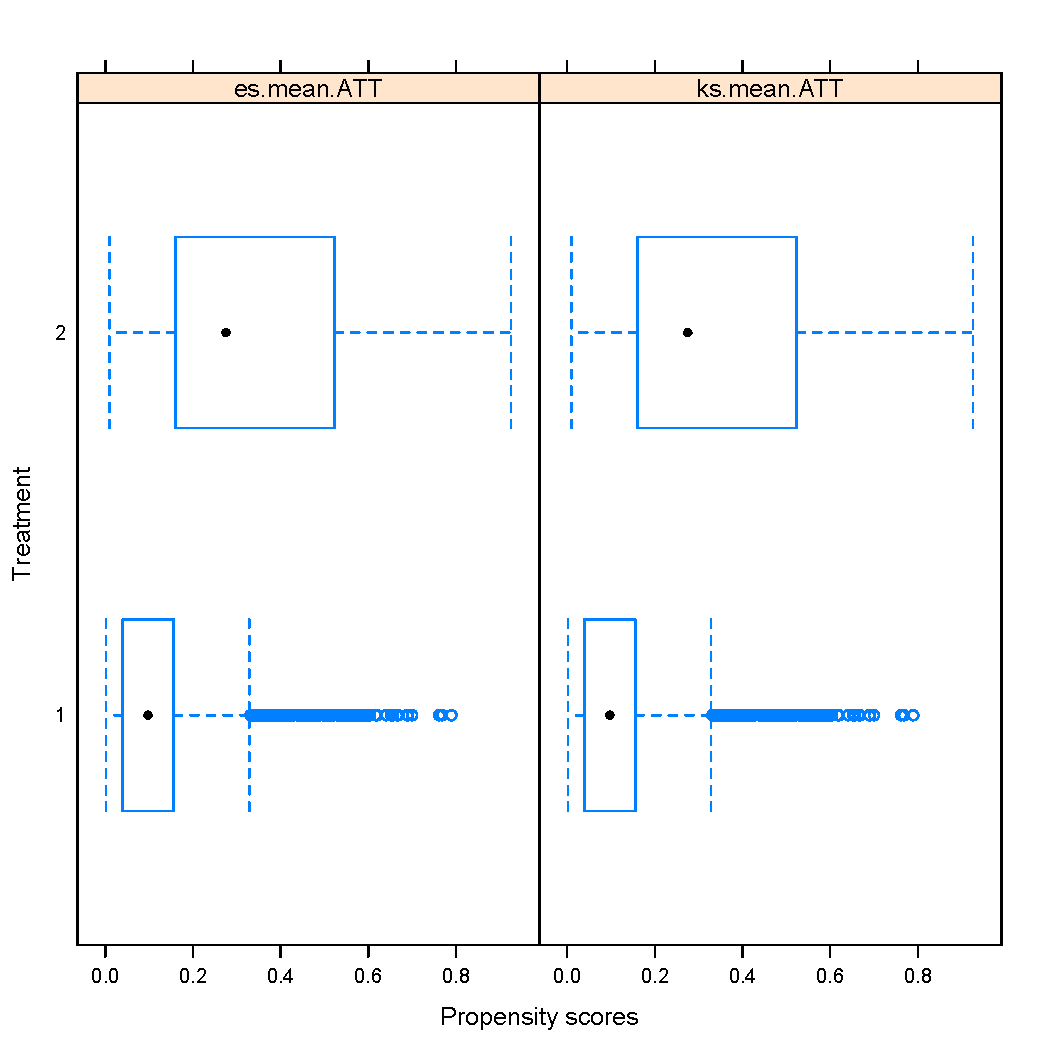
\includegraphics[width=\textwidth]{./figs/taf_jfk_twang_boxplot_pscores.pdf}
\caption{Propensity score distribution for treatment and control groups at JFK}
\label{fig:sil}
\end{figure}

\begin{figure}[h!]
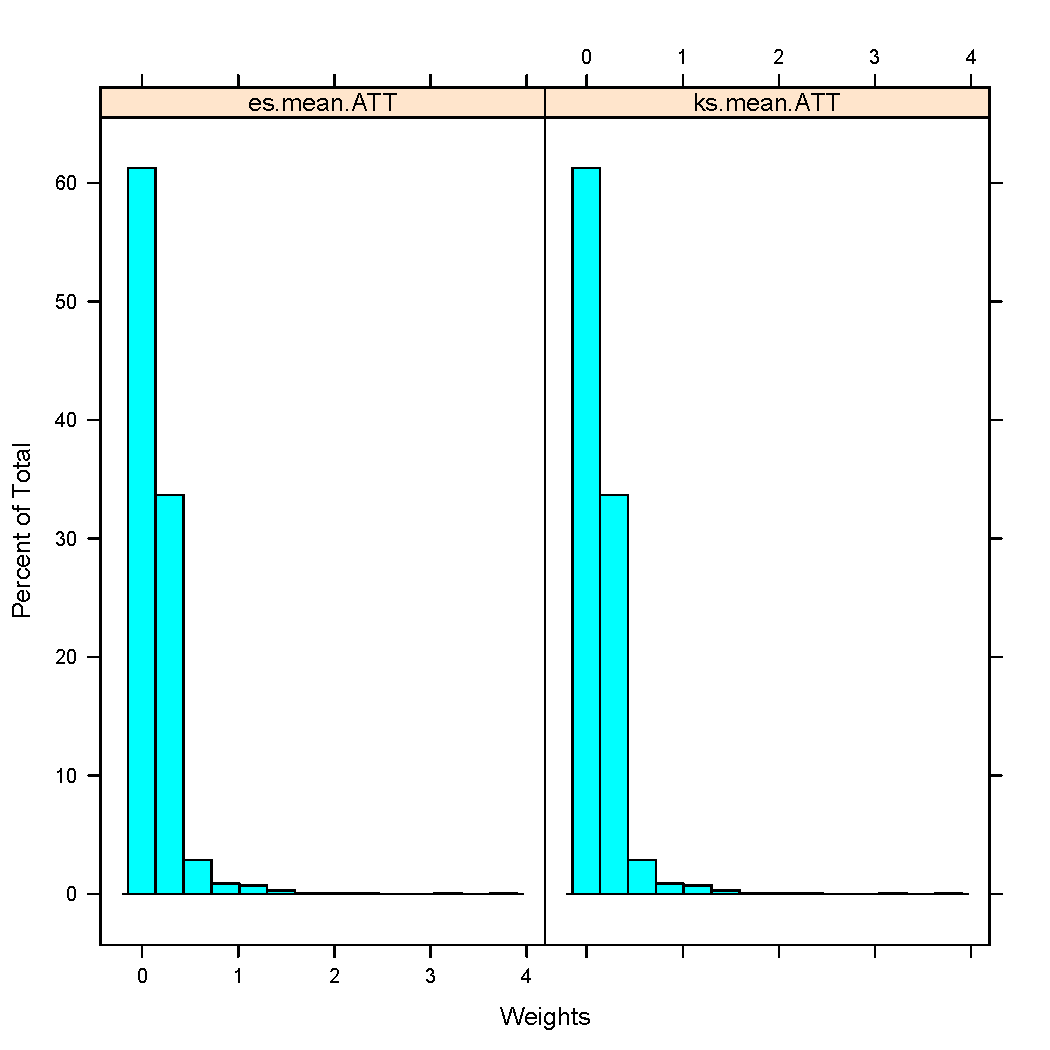
\includegraphics[width=\textwidth]{./figs/taf_jfk_twang_hist_weights.pdf}
\caption{IPTW weights distribution for JFK}
\label{fig:sil}
\end{figure}

\begin{figure}[h!]
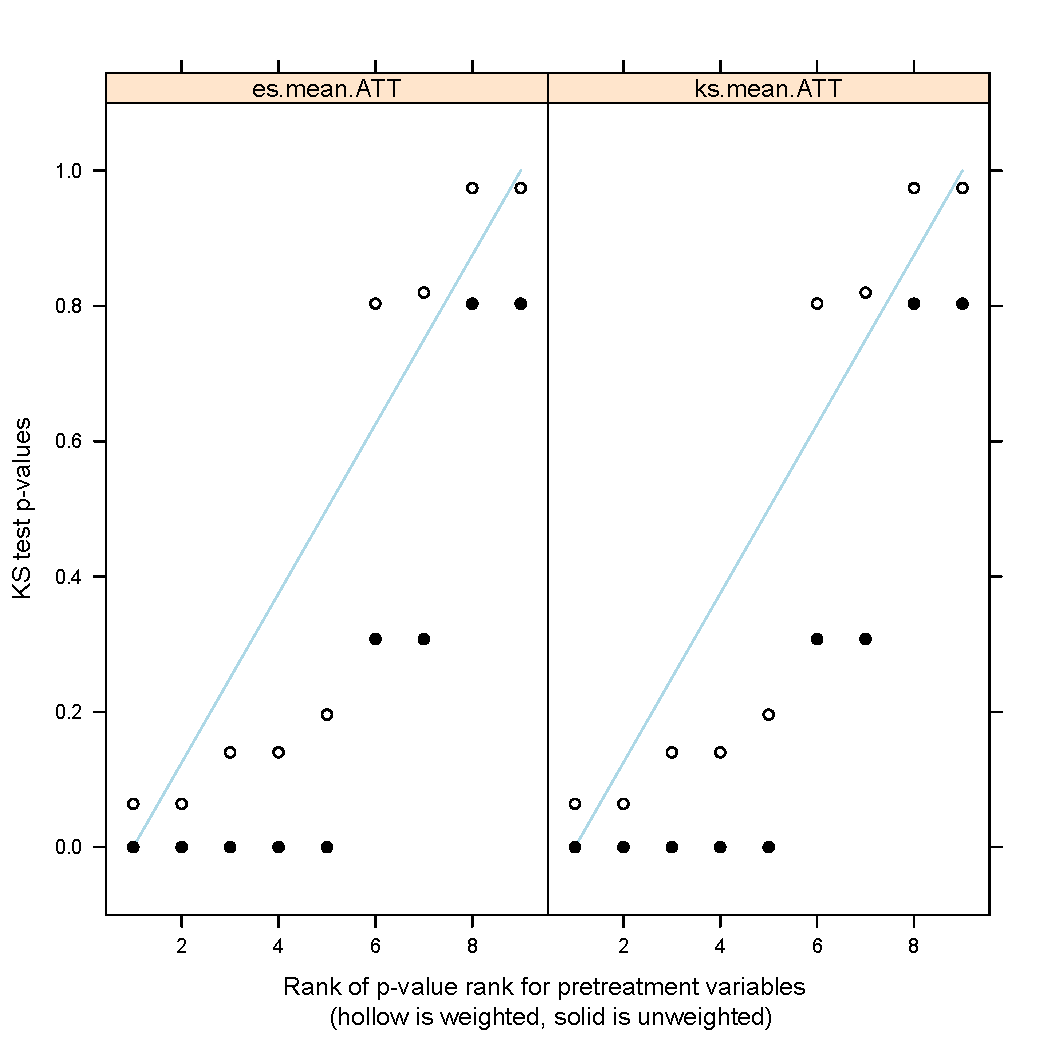
\includegraphics[width=\textwidth]{./figs/taf_jfk_twang_kstestPvals.pdf}
\caption{Balance improvement after IPTW reweighting for various confounding covariates at JFK}
\label{fig:sil}
\end{figure}

\begin{figure}[h!]
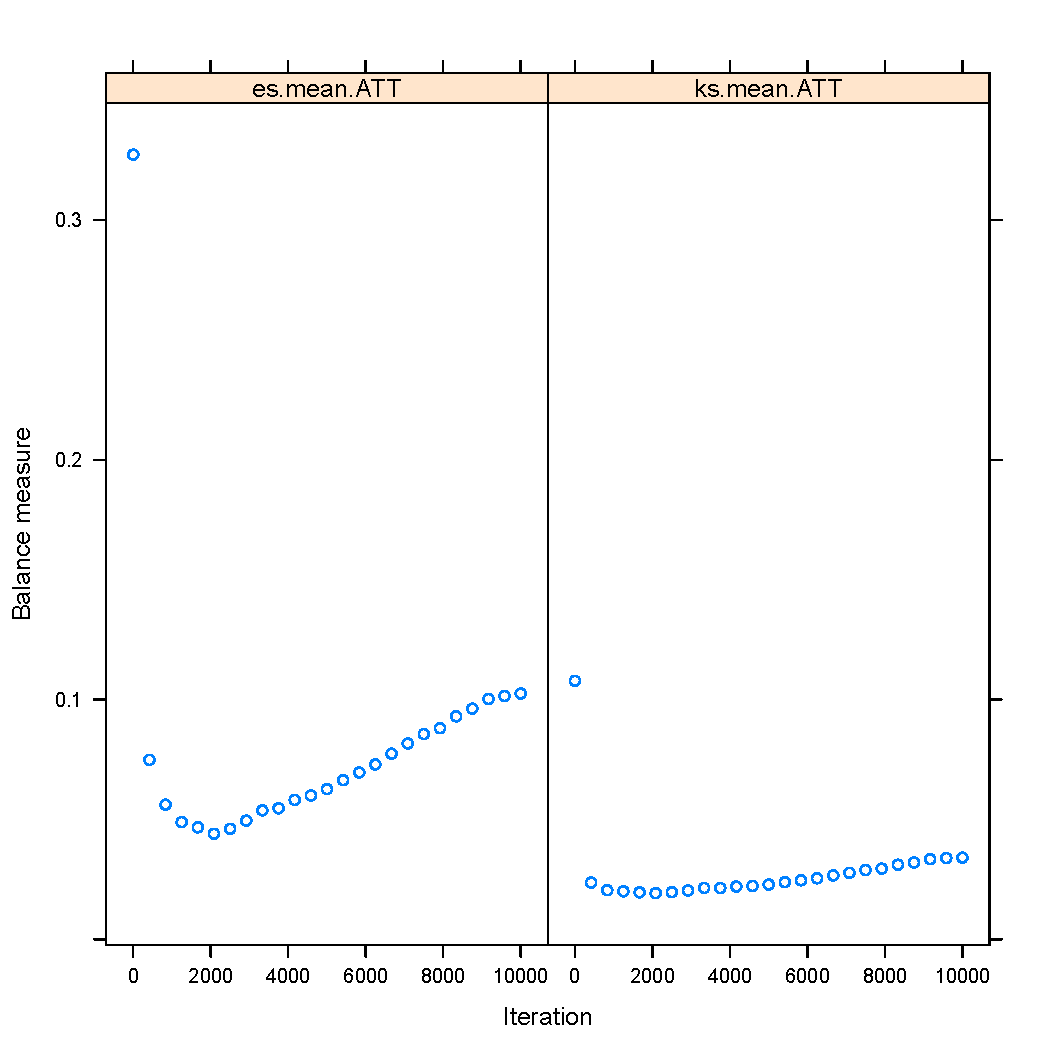
\includegraphics[width=\textwidth]{./figs/taf_twang_BalanceMeasureGBMiterations.pdf}
\caption{Propensity score model selection using the GBM algorithm with two different balance measure stopping criteria}
\label{fig:sil}
\end{figure}

Look at EWR

\newpage\noindent
\subsection*{EWR}
Now we consider EWR
%EWR
% latex table generated in R 3.1.0 by xtable 1.7-4 package
% Mon Feb 29 12:32:52 2016
\begin{table}[ht!]
\centering
\begin{tabular}{lrrr}
  \hline
 & E(Y1$|$t=1) & E(Y0$|$t=0) & p-value \\ 
  \hline
Crosswind & 9.91 & 8.00 & 0.00 \\ 
Visibility & 7.76 & 9.38 & -0.00 \\ 
No Snow & 0.95 & 0.98 & 0.00 \\ 
No Thunderstorms & 0.99 & 1.00 & 0.00 \\ 
No Rain & 0.77 & 0.94 & 0.00 \\ 
Arrivals & 34.62 & 32.26 & -0.00 \\ 
   \hline
\end{tabular}
\caption{Imbalance of the treatment and comparison groups for various weather and traffic (arrivals count) features (covariates) at EWR} 
\label{tab:imbalance}
\end{table}

% latex table generated in R 3.1.0 by xtable 1.7-4 package
% Mon Feb 29 12:39:25 2016
\begin{table}[ht!]
\centering
\begin{tabular}{lrrrr}
  \hline
 & E(Y1$|$t=1) & E(Y0$|$t=1) & p-value & E(Y0$|$t=0) \\ 
  \hline
Crosswind & 9.91 & 9.38 & 0.08 & 8.00 \\ 
Visibility & 7.76 & 8.14 & 0.04 & 9.38 \\ 
No Snow & 0.95 & 0.95 & 0.99 & 0.98 \\ 
No Thunderstorms & 0.99 & 1.00 & 0.00 & 1.00 \\ 
No Rain & 0.77 & 0.82 & 0.01 & 0.94 \\ 
Arrivals & 34.62 & 34.40 & 0.85 & 32.26 \\ 
   \hline
\end{tabular}
\caption{Simulated counterfactual E(Y0|t=1) and assessment of balance achieved by propensity score weighting the treatment and comparison groups using IPTW at EWR} 
\label{tab:balance}
\end{table}


\newpage\noindent

\bibliographystyle{plain}
\bibliography{gdp_causal}
\end{document}




























